\input sys/inputs.tex

\usepackage[utf8]{inputenc}
\usepackage[T1]{fontenc}
\usepackage[polish]{babel}
\usepackage{polski}

\begin{document}

\bigheading{Connect Highways}

% \info{task_name}{infile}{outfile}{points}{timelimit}{memlimit}
% leave this values, if you are not interested
\info{networks}{stdin}{stdout}{100}{400 ms}{32 MiB}

W~Bajtocji są dwie sieci autostrad kontrolowane przez dwie firmy: Czerwoną i Niebieską.
Obie sieci składają się ze skrzyżowań oraz z~dróg zbudowanych w~linii prostej między skrzyżowaniami, zwanych segmentami.
Sieci te są rozłączne.
Każdy segment i skrzyżowanie należy do dokładnie jednej firmy.
Segmenty się nie przecinają, co znaczy, że mogą się stykać tylko na skrzyżowaniach.
Dodatkowo, obie sieci są spójne, czyli między każdymi dwoma skrzyżowaniami należącymi do tej samej firmy,
	istnieje droga składająca się z~segmentów tej firmy.
Teraz, firmy te postanowiły złączyć się w~jedną.
Mają zamiar zbudować drogę w~linii prostej między pewnymi dwoma skrzyżowaniami, po jednym z~obu sieci.
Nowa droga nie może przecinać żadnego istniejącego segmentu. 

\heading{Task}

Napisz program, który znajduje odpowiedni segment łączący sieci obu firm.

\heading{Input}

Wejście zawiera kolejno opis sieci Czerwonej, a następnie Niebieskiej.
Pierwsza linia opisu sieci zawiera dwie liczby całkowite $N$ i $M$
	($2 \le N \le 200\,000$, $1 \le M \le 700\,000$), gdzie $N$ oznacza liczbę skrzyżowań, a $M$ oznacza liczbę segmentów.
W~kolejnych $N$ liniach znajdują się po dwie liczby całkowite $x$ i $y$
	($-1\,000\,000 \le x, y \le 1\,000\,000$), oznaczające współrzędne skrzyżowania.
W~kolejnych $M$ liniach znajdują się po dwie liczby całkowite $p$ i $q$ ($1 \le p, q \le N$, $p \neq q$), 
	oznaczające, że istnieje segment łączący skrzyżowania numer $p$ i $q$.
Skrzyżowania są ponumerowane od $1$ wzwyż w~kolejności, w~której pojawiły się na wejściu.

W~$30\%$ testów zachodzi $N, M \le 3000$.

\heading{Output}

W~pierwszym i jedynym wierszu wyjścia Twój program powinien wypisać dwie liczby całkowite $u$ i $v$,
	gdzie $u$ jest numerem skrzyżowania należącego do sieci Czerwonej,
	$v$ jest numerem skrzyżowania należącego do sieci Niebieskiej oraz segment łączący te skrzyżowania nie przecina
	żadnego innego segmentu.
Jeżeli istnieje wiele rozwiązań, Twój program powinien wypisać dowolne z~nich.

\heading{Sample}

\sampleIN
5 6
0 3
1 1
6 0
5 3
9 8
1 2
1 3
4 3
3 5
1 5
2 3
4 4
6 4
4 4
4 2
2 3
1 2
4 2
2 3
3 4
\sampleOUT
5 1
\sampleCOMMENT
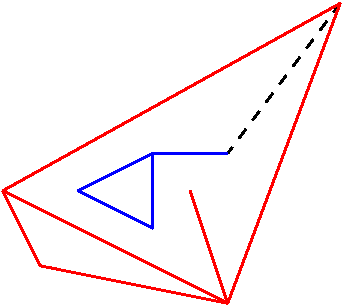
\includegraphics[height=4cm]{img/fig11.pdf}
\sampleEND

\end{document}
